\documentclass[11pt]{amsart}
\usepackage{amssymb, amsmath, mathptmx, graphicx, multicol, footmisc, graphicx, comment, textcomp, bm, color}
\usepackage{amscd}
\usepackage{amsfonts}
\usepackage{soul,xcolor,mathtools}

\usepackage[sc,osf]{mathpazo}

%STICKERS
%\usepackage{eso-pic}
%\newcommand\AtPagemyUpperLeft[1]{\AtPageLowerLeft{
%\put(\LenToUnit{0.9\paperwidth},\LenToUnit{0.9\paperheight}){#1}}}
%\AddToShipoutPictureFG{
%  \AtPagemyUpperLeft{{\includegraphics[width=.5in,keepaspectratio]{Expert.jpg}}}
%}

\newtheorem{definition}{Definition}
\newtheorem{example}{Example}
\newtheorem{theorem}{Theorem}
\newtheorem{exercise}{Exercise}
\newtheorem{lemma}{Lemmma}

\usepackage[colorlinks = true,
            linkcolor = blue,
            urlcolor  = blue,
            citecolor = blue,
            anchorcolor = blue]{hyperref}


\setcounter{MaxMatrixCols}{30}
\setlength{\topmargin}{-.5in}
\setlength{\textheight}{8.75in}
\setlength{\oddsidemargin}{-0.2in}
\setlength{\evensidemargin}{-0.2in}
\setlength{\textwidth}{6.5in}
\def\labelenumi{\arabic{enumi}.}
\def\theenumi{\arabic{enumi}}
\def\labelenumii{(\alph{enumii})}
\def\theenumii{\alph{enumii}}
\def\p@enumii{\theenumi.}
\def\labelenumiii{\arabic{enumiii}.}
\def\theenumiii{\arabic{enumiii}}
\def\p@enumiii{(\theenumi)(\theenumii)}
\def\labelenumiv{\arabic{enumiv}.}
\def\theenumiv{\arabic{enumiv}}
\def\p@enumiv{\p@enumiii.\theenumiii}
\newcommand{\ve}{\varepsilon}
\newcommand{\C}{\mathbb{C}}
\newcommand{\R}{\mathbb{R}}
\newcommand{\N}{\mathbb{N}}
\newcommand{\Q}{\mathbb{Q}}
\newcommand{\Z}{\mathbb{Z}}
\newcommand{\ds}[1]{\displaystyle{ #1}}
\newcommand{\tr}{\textrm{tr}}
\newcommand{\seq}[1]{(#1_n)_{n=1}^{\infty}}
\newcommand{\ser}[1]{\sum_{n=1}^{\infty} #1_n}
\renewcommand{\vec}[1]{\mathbf{#1}}

\newcommand{\normal}{\trianglelefteq}
\newcommand{\mbf}{\mathbf}
\newcommand{\mbb}[1]{\mbox{\boldmath$#1$}}
\newcommand{\con}{\, | \,}
\newcommand{\ip}[2]{\left\langle #1, #2 \right\rangle}
\newcommand{\der}[2]{\ds{\frac{\partial #1}{\partial#2}}}
\newcommand{\se}[1]{\setlength{\extrarowheight}{#1}}
\newcommand{\G}[2]{\ds{\Gamma_{#1}^{#2}}}
\newcommand{\wtilde}{\widetilde}
\newcommand{\surface}{$\vec{r} : \mathcal{U} \to \mathbb{R}^3$}
\newcommand{\WTS}{\xRightarrow[]{\text{WTS}}}

\pagestyle{plain}
\setcounter{secnumdepth}{0}
\parindent=0pt

\newcommand{\oscar}[1]{\textcolor{red}{\textbf{#1}}}
\setstcolor{red}
%\st{Some overstruck text}

\begin{document}

\begin{center}
\textbf{MATH 111, Assignment 1 Solutions}%CHANGE THIS EVERY WEEK
\end{center}

\vspace{.3 in}

\textbf{Name:}\underline{Dillon Allen} \hspace{1in} \textbf{Date:} \underline{August 26, 2021}%CHANGE THIS EVERY WEEK

\textbf{Group Name:}\underline{N/A}

\vspace{.3in}

\begin{enumerate}

\item Typeset the following text using LaTeX.

\vspace{.3in}
Many graphs contain substructures that may give information about their 'host' graph; One such substructure is a cycle.

\begin{definition}
	A sequence of distinct vertices $x_1, x_2, \ldots, x_k$ for all $i = 1, \ldots k$, and edges $e_1, e_2, \ldots, e_k$, such that each edge $e_i = x_i x_{i+1}$ is called a path. If we allow $x_1$ and $x_{k+1}$ to be the same vertex, then the path is said to be a cycle.
\end{definition}

\begin{example}
In $K_7$, consider the sequence of edges, $ x_1 x_2, x_2 x_3, x_3 x_1 $, whcih forms a 3-cycle that can be seen as the highlighted triangle in Figure 1.
\end{example}
\begin{center}
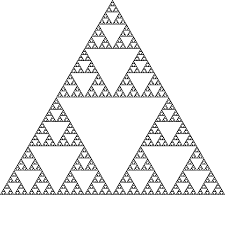
\includegraphics[height=1in]{sierpinski_triangle.png}
\end{center}

\begin{lemma}
All cycles contained in the Heawood graph must be of even length.
\end{lemma}

\begin{proof}
We provide a proof by contradiction, let $x_i$ be a vertex of $C_{14}$ and assume that the Heawood graph contains a cycle of odd length, denoted by $C = x_1 x_2 \ldots x_k x_1$. Since $C$ is an odd-length cycle, then $k$ must be odd. Since the Heawood graph is bipartite, then all vertices can be partitioned into two disjoint and pairwise non-adjacent sets $U,V$. Since $x_i$ and $x_{i+1}$ are adjacent, without loss of generality, suppose that $x_i \in U$ and $x_{i+1} \in V$, for all $i$ odd. Hence $\lbrace x_1, x_3, \ldots , x_k \rbrace \subseteq U$ and $\lbrace x_2, x_4, \ldots, x_{k-1} \rbrace \subseteq V$. Note that $x_k, x_1$ are adjacent in $C$, but $x_1$ and $x_k$ are both in $U$, contradicting that $U$ is pairwise non-adjacent. Thus the Heawood graph does not contain a cycle of odd length.
\end{proof}

\newpage

\item Type the following text into LaTeX (problem 2).

\vspace{.3in}

With this lemma, we can now prove the following two theorems. Since in our study we only deal with finite fields, it is enough to prove the Frobenius map is an automorphism if $F$ is finite.

\begin{theorem}
Let $p$ be prime and $F$ a field such that $char\left(F\right) = p$. Then, 
\[
	\phi : F \to F : x \mapsto x^p
\]
is an automorphism.
\end{theorem}

\begin{proof}
Using the Binomial Theorem, we have that $\left(a + b\right)^p = a^p + b^p$ and so
\[
	\phi\left(a + b\right) = \phi\left(a\right) + \phi\left(b\right)
\]
Since $F$ is a field, then all elements in $F$ commute, which implies that $\left(ab\right)^p = b^p a^p = a^p b^p$. Hence, this gives us that $\phi\left(ab\right) = \phi\left(a\right) \phi\left(b\right)$. Therefore, $\phi$ is a homomorphism of fields. Suppose $F$ is finite, Now, let $x \in F$ and suppose $x \in Ker \left(\phi\right)$. Then, we can see that

\begin{align*}
	x \in Ker\left(\phi\right) &\iff \phi\left(x\right) = 0_{F} \\
							   &\iff x^p = 0_F \\
							   &\iff x = 0_F ,
\end{align*}
where the last equation follows from $F$ not containing any zero divisors. This, since $F$ is finite and $\phi$ is injective then by the 2-out-of-3 property, $\phi$ is bijective.
\end{proof}

\begin{theorem}
	Every element in $F_q$ is a solution of the equation $x^q = x$.
\end{theorem}

\begin{proof}
	We have the $\lvert F_q \rvert = q = p^n$, for some prime $p$, and $n \in \mathbb{N}$. Suppose that $x \in F_q$. We will consider the following two cases.
	
	(Case 1) Suppose that $x = 0_{F_q}$. Then, it is easy to see that $x^{p^n} = x$.
	
	(Case 2) Suppose that $x \neq 0_{F_q}$. Then, $x \in F^{\ast}_{q}$. Since $F_q$ is a finite field, then $F^{\ast}_q$ is the multiplicative group with $\lvert F^{\ast}_q \rvert = q - 1 = p^n - 1$. Since $F^{\ast}_q$ is a finite group, then $x^{\lvert F^{\ast}_q \rvert} = 1_{F_q}$; and thus, $x^{p^n - 1} = 1_{F_q} $. By multiplying both sides by $x$, we get $x^{p^n} = x$. Therefore, $x^q = x$. 
\end{proof}

Now, we embark on our study of field extensions by first introducing some basic definitions and results.

\begin{definition}
	If $K$ is a field containing a subfield $F$, then $K$ is a field extension of $F$ which will be denoted as $K / F $.
\end{definition}

\end{enumerate}
%
%\begin{definition}
%This is a command I created: $\WTS$. Use it.
%\end{definition}
%
%\begin{theorem}
%This is a theorem.
%\end{theorem}
%
%\vspace{.3in}
%
%\begin{enumerate}
%
%\item HERE GOES THE STATEMENT OF PROBLEM 1
%
%\begin{proof}
%HERE GOES THE SOLUTION/PROOF TO PROBLEM 1
%\end{proof}
%
%\vspace{.1in}
%
%\item HERE GOES THE STATEMENT OF PROBLEM 2
%
%\begin{proof}
%HERE GOES THE SOLUTION/PROOF TO PROBLEM 2
%\end{proof}
%
%
%
%
%
%
%\vspace{1in}
%
%
%
%
%
%
%\noindent \textbf{HW reminders.}
%\begin{enumerate}
%\item For Assignments 1 and 2, please submit a pdf file to CANVAS and email me the corresponding tex file by the deadline. Starting in assignment 3, there is no need to submit a tex file to me, just the pdf to CANVAS. 
%
%\item You need to create a group contract by the time HW 2 is due. You do not need to resend this unless changes in your group happen.
%
%\item Please email me weekly your individual weekly report (every week).
%
%\item Please make a copy of this file to write your assignment's solutions. Making changes to it, or to use a different file will create problems.
%\end{enumerate}
%\end{enumerate}
%
%
%
%
%
%
%
%
%\newpage
%
%
%
%
%\begin{itemize}
%\item How to get parentheses, brackets of the right size? Use left and right before them. For example
%\[
%\left(\frac{1}{3}\right)^2 =\frac{1}{9}
%\]
%For curly brackets, it is a little more complicated. You need to use an extra backslash
%\[
%A = \left\{   \frac{1}{3}, \frac{1}{9}    \right\}
%\]
%
%\item The natural numbers, rationals, reals, and complex numbers have special shortcuts: $\N$, $\Q$, $\R$, $\C$.
%
%\item This is OK: $\int_0^1 f(x) \ dx$, but this is better $\ds{\int_0^1 f(x) \ dx}$. You could also do
%\[
%\int_0^1 f(x) \ dx
%\]
%
%\item Similarly,  this is OK: $\lim_{n\to \infty} a_n$, but this is better $\displaystyle{\lim_{n\to \infty} a_n}$. And as an equation, we get
%\[
%\lim_{n\to \infty} a_n
%\]
%
%\item There are more examples of how to do things in the \LaTeX \ workshop file posted on CANVAS.
%\end{itemize}







\end{document}